\problemname{High Noon}

Ready up, cowboy. 

You have a duel at high noon (12 o'clock in the middle of the day, or 12 pm). 
Make sure you are here on time to shoot your shot.

\begin{centering}
  \begin{figure}[h]
      \centering
      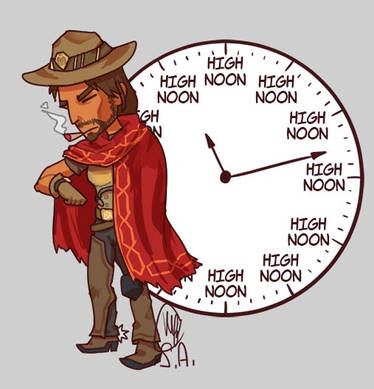
\includegraphics[width=0.8\textwidth]{highnoon.jpg}
      \caption{"Local Man Tells the Time" by essuei, from \href{https://www.deviantart.com/essuei/art/Overwatch-Local-Man-Tells-the-Time-614496598}{www.deviantart.com}. Licensed under \href{https://creativecommons.org/licenses/by-nc-nd/3.0/}{CC BY-NC-ND 3.0 DEED}.}
  \end{figure}
\end{centering}

\section*{Input}
There is no input. Just make sure you are ready.

\section*{Output}
Write ``PANG!'' on a single line to shoot your shot.

\section*{Grading}
\textbf{Note:} You can only submit \textbf{one} correct solution för detta problem. If you already have submitted a correct solution, then only the first submission will count. 
You can get from 0 up to 100 points. If you submit exactly at \href{https://www.timeanddate.com/worldclock/fixedtime.html?msg=Ready+yourself%2C+Cowboy&iso=20240401T12&p1=239}{High Noon} 
($12:00:00$ Swedish time), then you get 100 poäng. For every second away from $12:00:00$ you submit, you will recieve 1 point less. 

For example if you submit at $11:59:55$, you will only get $95$ points. If you submit at $12:01:00$, you will only get $40$ points.
But if you submit at $11:30:00$ you will get $0$ points.

